% gesture_mimic.tex
% GTAC 2026 double-blind submission
% Content: Real-time imitation learning for gesture mimicry on AMD hardware.

\documentclass[blind]{gtac}

\usepackage{cite}
\usepackage{xcolor}
\usepackage{booktabs}
\usepackage{amsmath}
\usepackage{amssymb}
\usepackage{float}
\usepackage{tikz}
\usetikzlibrary{arrows.meta,positioning,calc}
\usepackage{algorithm}
\usepackage{algpseudocode}
\usepackage[colorlinks=true, linkcolor=blue, urlcolor=blue, citecolor=blue]{hyperref}
\Urlmuskip=0mu plus 1mu\relax % allow long URLs in references to break

\SetWatermarkScale{0.3}
\SetWatermarkAngle{30}
\SetWatermarkColor{gray!20}

\title{Is Acceleration the New Accuracy? Real-Time Imitation Learning for
Gesture Mimicry with a Compact Vision-Language-Action Policy on AMD Hardware}

\author{Anonymous}

\begin{document}

\maketitle

\pagestyle{fancy}
\fancyhf{}
\cfoot{\thepage}
\renewcommand{\headrulewidth}{0pt}
\chead{{\sffamily\textcolor{red}{\fontsize{10}{12}\selectfont\textbf{DO NOT FORWARD -- FOR GTAC'26 REVIEW COMMITTEE ONLY}}}}
\thispagestyle{fancy}

\begin{abstract}
Vision-Language-Action (VLA) policies trained by imitation learning have made
general-purpose robot control practical, but their real-world usefulness is
gated less by peak accuracy than by \emph{latency}: a policy that predicts the
right motion too late produces the wrong motion. We study this coupling on a
reactive \emph{gesture-mimicry} task, in which an SO-101 robot arm running on
LeRobot must imitate a human's hand and wrist gestures observed through a single
camera in real time. We fine-tune the compact 450M-parameter SmolVLA policy by
behavior cloning on 2{,}000 teleoperated master--slave demonstrations collected
from multiple people and backgrounds, and evaluate it by mean absolute error
(MAE) between predicted and ground-truth joint trajectories. Because the policy
emits chunks of 50 future actions from a single observation, we show---both
analytically and empirically---that consuming more actions from a stale chunk
before re-observing collapses accuracy (MAE grows from 3.3 at one action to
23.1 at forty), so the only way to stay accurate is to re-observe often, which
in turn demands low inference latency. We then close the latency gap on AMD
GPU (Strix/GPK-class) hardware through a sequence of systems optimizations:
reducing flow-matching denoising steps from 30 to 2, compiling the full
encoder-plus-prefill graph (not merely the denoiser) with \texttt{torch.compile},
casting to FP16 \emph{before} compilation to avoid ROCm rescaling overhead,
reducing the three-camera input to the single camera the task actually uses, and
running Real-Time Chunking (RTC) asynchronous inference with a lowered refill
threshold. Together these deliver roughly a $7\times$ throughput increase (2 to
13--15 inferences/s) and a $\sim$50\% MAE reduction (6 to $\sim$3, under the
$\sim$3.5 usability limit), turning an unusable policy into a smooth, deployable
one. The result is a concrete demonstration that on AMD hardware, systems-level
acceleration is a direct and measurable driver of task accuracy for reactive
embodied AI.
\end{abstract}

\keywords{imitation learning, vision-language-action models, SmolVLA, action
chunking, real-time inference, flow matching, ROCm, torch.compile, robot
learning, edge AI.}

%---------------------------------------------------------------------------
\section{Introduction}
\label{sec:intro}
%---------------------------------------------------------------------------

Recent Vision-Language-Action (VLA) models adapt pretrained vision-language
backbones into robot policies that map camera images and a language instruction
to low-level motor commands~\cite{rt2,openvla,pi0,smolvla}. Trained by imitation
learning on teleoperated demonstrations, they generalize across objects and
tasks far better than per-task policies. Yet a property that is easy to overlook
in benchmark tables becomes decisive on a physical robot: a VLA is a
\emph{closed-loop} system, and its usefulness depends not only on \emph{what} it
predicts but on \emph{when} the prediction arrives. A policy that computes the
correct action for the world it saw 300\,ms ago is, on a moving target, simply
wrong.

We make this coupling concrete on a deliberately unforgiving task:
\textbf{gesture mimicry}. A human stands in front of a single camera and moves a
hand up/down and left/right and opens or closes the wrist; an SO-101 arm running
on the LeRobot stack~\cite{lerobot} must \emph{mimic} the gesture as it happens.
Unlike pick-and-place, the target is a live, continuously moving human, so there
is no ``settling time'': every millisecond of policy latency is a millisecond of
lag between operator and robot. This makes gesture mimicry an ideal probe for the
thesis of this paper---that for reactive embodied AI, \textbf{acceleration is the
new accuracy}.

The mechanism behind the thesis is action chunking. Modern
VLAs~\cite{act,pi0,smolvla} predict a \emph{chunk} of $n$ future actions from one
observation to amortize inference cost and enforce temporal consistency. The more
of that chunk the robot executes before capturing a fresh observation, the
further it extrapolates open-loop from stale perception, and the worse it tracks
a moving target. The only remedy is to re-observe and re-predict often---which is
affordable only if each inference is fast. Latency and accuracy are therefore not
independent axes; on this task they are the same axis.

This paper contributes: (1) a reactive gesture-mimicry benchmark and a
2{,}000-episode master--slave imitation-learning dataset for the SO-101
(Section~\ref{sec:task}); (2) an empirical characterization of the
chunk-consumption effect, showing MAE degrading monotonically from 3.3 to 23.1
as more stale actions are executed, mirroring the SmolVLA
paper's own ablation and establishing the speed--accuracy identity
(Section~\ref{sec:speed}); (3) a description of the Real-Time Chunking
asynchronous control loop that exploits low latency to keep the action queue
fresh (Section~\ref{sec:rtc}); and (4) a sequence of AMD-specific systems
optimizations---diffusion-step reduction, full-graph \texttt{torch.compile},
compile-aware FP16, single-camera reduction, and RTC tuning---that yield $\sim
7\times$ throughput and $\sim$50\% lower MAE on Strix/GPK-class hardware, taking
the policy from unusable to deployable (Sections~\ref{sec:amd}--\ref{sec:results}).

%---------------------------------------------------------------------------
\section{Background and Related Work}
\label{sec:background}
%---------------------------------------------------------------------------

\textbf{Imitation learning and action chunking.}
Behavior cloning learns a policy $\pi_\theta(a\mid o)$ directly from
expert demonstrations $(o,a)$, but small per-step errors compound over a
trajectory~\cite{act}. Action Chunking with Transformers (ACT) mitigates this by
predicting a short sequence of future actions as one unit, reducing the effective
horizon over which errors accumulate and improving temporal
smoothness~\cite{act}. Chunking is now standard across VLAs~\cite{pi0,smolvla},
but it introduces the very staleness problem we study: a chunk predicted from
$o_t$ is executed over timesteps $t\!:\!t\!+\!n$, during which the world moves on.

\textbf{Generative action heads.}
Rather than regressing a single action, recent policies model the action
distribution with diffusion~\cite{diffusionpolicy} or flow
matching~\cite{flowmatching}, which capture multimodality and produce smooth
trajectories. $\pi_0$~\cite{pi0} and $\pi_{0.5}$~\cite{pi05} attach a
flow-matching ``action expert'' to a pretrained VLM; SmolVLA~\cite{smolvla}
follows the same recipe at a fraction of the size. The cost is an iterative
denoising loop at inference time, which is a primary latency contributor and a
main target of our optimization (Section~\ref{sec:amd}).

\textbf{Compact VLAs.}
Where OpenVLA~\cite{openvla} (7B) and $\pi_0$~\cite{pi0} (3.3B) are large,
SmolVLA~\cite{smolvla} is a 450M-parameter open policy built on the efficient
SmolVLM-2 backbone~\cite{smolvlm} and trained on community
data, explicitly targeting single-GPU training and consumer-grade deployment.
Its small size is what makes aggressive real-time optimization on a single AMD
GPU tractable, so we adopt it as our base policy.

\textbf{Real-time execution.}
Black et al.~\cite{rtc} formalize the latency problem and propose Real-Time
Chunking (RTC): generate the next chunk while executing the current one, freezing
the actions that will certainly run and ``inpainting'' the overlap for
continuity. SmolVLA~\cite{smolvla} ships a complementary asynchronous inference
stack that decouples action execution from prediction. Our deployment builds on
the LeRobot~\cite{lerobot} implementation of these ideas and studies how far
low latency, achieved through AMD systems optimization, extends their benefit.

%---------------------------------------------------------------------------
\section{The Gesture-Mimic Task and Dataset}
\label{sec:task}
%---------------------------------------------------------------------------

\subsection{Task Definition}

A human operator performs hand gestures---raising and lowering the arm, moving
left and right, and opening or closing the wrist---in front of a single RGB
camera. The policy observes the camera frame and the arm's current joint state
and must drive an SO-101 6-DoF arm so that its end-effector pose mirrors the
human's gesture in real time (Figure~\ref{fig:loop}). The task is purely
reactive: there is no goal object and no fixed end state, so quality is measured
by how faithfully and how promptly the arm tracks the live gesture.

\begin{figure}[H]
\centering
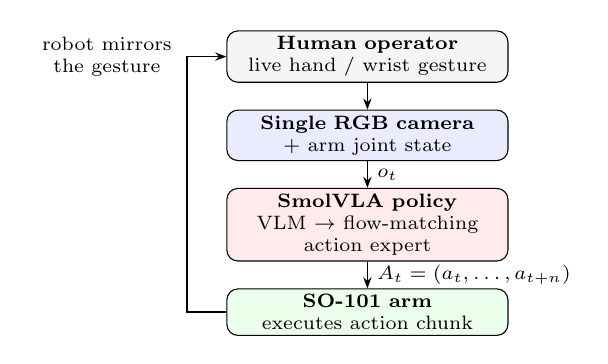
\begin{tikzpicture}[
  font=\scriptsize,
  node distance=3.4mm,
  box/.style={draw, rounded corners, align=center, text width=1.35in,
              minimum height=3.0ex, inner sep=2pt},
  human/.style={box, fill=gray!8},
  sense/.style={box, fill=blue!8},
  model/.style={box, fill=red!8},
  act/.style={box, fill=green!8},
  arr/.style={-{Stealth[length=1.4mm]}, semithick}
]
\node[human] (h) {\textbf{Human operator}\\ live hand / wrist gesture};
\node[sense, below=of h] (cam) {\textbf{Single RGB camera}\\ + arm joint state};
\node[model, below=of cam] (vla) {\textbf{SmolVLA policy}\\ VLM $\to$ flow-matching\\ action expert};
\node[act, below=of vla] (arm) {\textbf{SO-101 arm}\\ executes action chunk};
\draw[arr] (h) -- (cam);
\draw[arr] (cam) -- node[right]{$o_t$} (vla);
\draw[arr] (vla) -- node[right]{$A_t=(a_t,\dots,a_{t+n})$} (arm);
\draw[arr] (arm.west) -- ++(-0.5,0) |- (h.west)
      node[midway,left,text width=0.7in,align=center]{robot mirrors\\ the gesture};
\end{tikzpicture}
\caption{The gesture-mimic closed loop. A single camera observation $o_t$ drives
the SmolVLA policy, which emits a chunk of $n$ future actions executed by the
SO-101 arm. Because the operator moves continuously, any latency between
observation and execution appears directly as tracking lag.}
\label{fig:loop}
\end{figure}

\subsection{Data Collection by Master--Slave Teleoperation}

We collect demonstrations by imitation learning in the classic teleoperation
setup~\cite{act}. The arm ships as a \emph{master}--\emph{slave} pair connected
by a cable: a human moves the master arm while watching the person in front of
the camera, and the slave arm's motors reproduce the master's joint positions
exactly. We record the camera video together with the synchronized slave-arm
joint trajectory; time-aligning the two yields
$(\text{image}\rightarrow\text{action vector})$ pairs. Because the demonstrated
action is the operator's own gesture-tracking motion, the learned policy directly
imitates human gesture-mimicking behavior---textbook behavior cloning.

The corpus comprises \textbf{2{,}000 episodes} spanning multiple demonstrators
and varied visual backgrounds, aggregated from several LeRobot-format datasets.
Validation uses a held-out set of 10 seen-speaker episodes. We report
\textbf{mean absolute error (MAE)} between predicted and ground-truth joint
trajectories (lower is better); qualitatively, motion becomes visibly unusable
above an MAE of roughly \textbf{3.5}, which we treat as the usability threshold.

%---------------------------------------------------------------------------
\section{Policy Architecture}
\label{sec:model}
%---------------------------------------------------------------------------

We fine-tune SmolVLA~\cite{smolvla}, whose two components are summarized here
because they set up the latency budget we later attack.

\textbf{Perception (VLM).} A SmolVLM-2 backbone~\cite{smolvlm} (SigLIP vision
encoder + SmolLM2 decoder) encodes the concatenation of image tokens, the
language instruction, and a single state token obtained by linearly projecting
the joint proprioception. Three efficiency choices make it small and fast:
each frame is compressed to \textbf{64 visual tokens} via pixel shuffle; only the
\textbf{first $N=L/2$ (16) decoder layers} are used to condition control; and the
action expert interleaves \textbf{cross-attention} (to the VLM's cached keys and
values) with \textbf{causal self-attention} over action tokens.

\textbf{Control (action expert).} A $\sim$100M-parameter flow-matching
Transformer~\cite{flowmatching,pi0} of width $0.75\times$ the VLM hidden size
predicts an action chunk $A_t=(a_t,\dots,a_{t+n})$ with $n=50$. Inference
integrates a learned velocity field over a small number of denoising steps
(default 10). The VLM prefix is encoded once and cached; the denoising loop
reuses that cache. This structure means inference latency has two parts---a
\emph{one-time prefix/encoder cost} and a \emph{per-step denoising cost}---both
of which we reduce in Section~\ref{sec:amd}.

%---------------------------------------------------------------------------
\section{Speed Is the New Accuracy}
\label{sec:speed}
%---------------------------------------------------------------------------

\subsection{Why Consuming a Chunk Hurts Accuracy}

A chunk $A_t$ is predicted from a single observation $o_t$. If the robot executes
$k$ actions from $A_t$ before capturing a new observation, then action $a_{t+k}$
is applied to a world that has advanced $k$ control periods past $o_t$. On a
static task this open-loop extrapolation is cheap; on a live gesture it is
corrosive, because the human has moved and the late actions track a pose that no
longer exists. Accuracy therefore degrades monotonically with the number of
\emph{consumed} (stale) actions.

Table~\ref{tab:actionstates} shows exactly this on our validation set (SmolVLA
v1, FP16, $\sim$65\,ms latency). MAE is 3.28 when a single fresh action is
consumed per inference and climbs to 23.07 at forty---an $\sim\!7\times$
degradation driven purely by staleness, not by any change in the model. The
SmolVLA paper reports the same qualitative collapse in its execution-horizon
ablation (success rate $80.3\%\!\rightarrow\!51.8\%$ as executed actions grow
from 1 to 50)~\cite{smolvla}; our continuous MAE metric makes the effect even
sharper.

\begin{table}[H]
\centering
\caption{MAE versus number of consumed (stale) action states, at fixed
$\sim$65\,ms latency (SmolVLA v1, FP16). Executing more of a chunk before
re-observing sharply worsens accuracy.}
\label{tab:actionstates}
\footnotesize
\begin{tabular}{@{}ccc@{}}
\toprule
Consumed actions & MAE & Latency (ms) \\
\midrule
1  & \textbf{3.28} & 65.16 \\
2  & 3.43 & 65.37 \\
4  & 4.29 & 67.72 \\
5  & 4.56 & 66.81 \\
10 & 4.80 & 65.00 \\
20 & 6.21 & 64.05 \\
30 & 12.09 & 62.83 \\
40 & 23.07 & 64.33 \\
\bottomrule
\end{tabular}
\end{table}

\subsection{The Latency--Reactivity Identity}

The practical consequence is that accuracy demands \emph{frequent re-observation},
and re-observation frequency is bounded by inference latency. Following the
asynchronous-inference analysis~\cite{rtc,smolvla}, to keep the action queue from
emptying (and thus keep the robot from either stalling or running open-loop) the
queue-refill threshold $g\in[0,1]$ must satisfy
%
\begin{equation}
g \;\ge\; \frac{\mathbb{E}[\ell_S]}{n\,\Delta t},
\label{eq:g}
\end{equation}
%
where $\ell_S$ is inference latency, $\Delta t$ the control period, and $n$ the
chunk size. Equation~\eqref{eq:g} states the identity plainly: \emph{lower
latency $\ell_S$ permits a smaller $g$}, i.e. fewer inferences to stay reactive,
or equivalently, at fixed $g$, a larger safety margin so the queue always holds
fresh actions. Either way, cutting $\ell_S$ directly buys the ability to consume
fewer stale actions per inference---which, by Table~\ref{tab:actionstates}, is
exactly what lowers MAE. This is why, on this task, \textbf{a faster model is a
more accurate model}. It is also why the fastest configuration in our sweeps is
consistently the most accurate one, even at fixed model weights: lower latency
lets the RTC loop overwrite stale actions with fresh predictions before they are
ever executed (Section~\ref{sec:rtc}).

%---------------------------------------------------------------------------
\section{Real-Time Chunking and Asynchronous Inference}
\label{sec:rtc}
%---------------------------------------------------------------------------

To turn low latency into fresh actions, we run the policy in an asynchronous
Real-Time Chunking loop~\cite{rtc,smolvla} rather than the naive
predict-then-execute-whole-chunk scheme. Execution and prediction are decoupled:
a control thread pops actions from a thread-safe queue at a fixed rate and never
blocks on the model, while an inference thread refills the queue in the
background from the latest observation. A new chunk is requested \emph{before}
the queue drains (when its remaining fraction falls below $g$), and the new chunk
is aggregated onto the unexecuted tail of the old one so motion stays continuous
across chunk boundaries. Actions rendered stale by the time the new chunk lands
are dropped by a latency-based delay of $\lceil \ell_S/\Delta t\rceil$ steps.
Algorithm~\ref{alg:rtc} sketches the loop.

\begin{algorithm}[H]
\footnotesize
\caption{Asynchronous Real-Time Chunking control loop}
\label{alg:rtc}
\begin{algorithmic}[1]
\State capture $o_0$; \; $A \gets \pi(o_0)$ \Comment{initial chunk}
\State $\textit{handle} \gets \textbf{null}$
\For{$t = 1 \dots T$}
  \State $a_t \gets \Call{PopFront}{A}$; \; \Call{Execute}{$a_t$}
  \If{$|A|/n < g$ \textbf{and} \textit{handle} is idle}
     \State capture $o_{t}$
     \If{\Call{NeedsProcessing}{$o_{t}$}} \Comment{skip near-duplicates}
        \State $\textit{handle} \gets \Call{AsyncInfer}{o_{t}}$ \Comment{non-blocking}
     \EndIf
  \EndIf
  \If{\textit{handle} completed}
     \State $\tilde{A} \gets$ result of \textit{handle}
     \State drop first $\lceil \ell_S/\Delta t\rceil$ actions of $\tilde{A}$
     \State $A \gets \Call{Aggregate}{A, \tilde{A}}$ \Comment{overlap the tail}
     \State $\textit{handle} \gets \textbf{null}$
  \EndIf
\EndFor
\end{algorithmic}
\end{algorithm}

The knob that matters for accuracy is the refill threshold $g$ (in our stack the
\texttt{chunk\_size\_threshold}). Lowering it makes the loop request fresh chunks
sooner, so each executed action is grounded in a more recent observation---but a
low $g$ is only \emph{affordable} when $\ell_S$ is small, per
Equation~\eqref{eq:g}. Our AMD optimizations shrink $\ell_S$; the RTC loop then
converts that headroom into reactivity, and reactivity into accuracy.

%---------------------------------------------------------------------------
\section{Systems Optimization on AMD Hardware}
\label{sec:amd}
%---------------------------------------------------------------------------

The base policy runs at $\sim$2 inferences/s in eager FP32---far too slow for
reactive mimicry. We reduce latency on a single AMD GPU (Strix/GPK-class,
ROCm~\cite{rocm}) through the sequence in Table~\ref{tab:ladder}. The upstream
release ships only bfloat16 plus \texttt{torch.compile} on the flow-matching
denoiser~\cite{smolvla,pytorch2}; our work extends the optimization to the whole
policy and to the ROCm-specific precision path.

\begin{table}[H]
\centering
\caption{Optimization ladder on a single AMD GPU. Each row is cumulative.}
\label{tab:ladder}
\footnotesize
\begin{tabular}{@{}p{1.55in}p{0.55in}p{0.55in}@{}}
\toprule
Optimization & Effect & Throughput \\
\midrule
Baseline (eager, FP32) & --- & 2.0 inf/s \\
Diffusion steps $30\!\to\!2$ & fewer expert passes & 4.5--5 inf/s \\
Full-graph \texttt{torch.compile} & fused kernels & 8.5 inf/s \\
FP16 cast \emph{before} compile & half compute & 13--15 inf/s \\
$3\!\to\!1$ camera input & less encode & speed + acc.\\
RTC + \texttt{chunk\_threshold}$\downarrow$ & fresher obs. & reactivity$\uparrow$ \\
Action smoothing (post) & de-jitter & smoothness$\uparrow$ \\
\bottomrule
\end{tabular}
\end{table}

\textbf{Diffusion steps $30\rightarrow2$.} For this task the flow-matching field
is well approximated in two integration steps; extra steps add latency without
measurable accuracy gain. This alone more than doubles throughput.

\textbf{Full-graph \texttt{torch.compile}.} We rewrote the LeRobot SmolVLA
modules so that the vision encoder and the LLM-prefix prefill compile into a
single graph~\cite{pytorch2}, not just the denoising step as
upstream. This removes per-layer Python dispatch and lets the compiler fuse
kernels across the whole forward pass, reaching $\sim$8.5 inf/s.

\textbf{Compile-aware FP16.} Casting weights to FP16 \emph{before} compilation is
critical on ROCm: casting afterwards makes the compiler insert up/down-scale
operations around every layer, and the resulting overhead eats the precision
win. Casting first yields a clean half-precision graph and pushes throughput to
13--15 inf/s. The best deployable configuration is FP16 with
max-autotune-no-cudagraphs full-graph compilation at $\sim$65\,ms standalone
latency (Table~\ref{tab:compile}); a one-time cold-start compilation cost is paid
once and cached.

\begin{table}[H]
\centering
\caption{Compile-mode comparison at 10 consumed actions. FP16 with full-graph
compilation gives the lowest latency.}
\label{tab:compile}
\footnotesize
\begin{tabular}{@{}llcc@{}}
\toprule
Precision & Compile mode & MAE & Latency (ms) \\
\midrule
FP16 & no-cudagraphs-full & 4.80 & \textbf{65.00} \\
FP16 & reduce-overhead & 4.60 & 77.20 \\
FP16 & eager & 5.02 & 85.61 \\
BF16 & reduce-overhead & 4.75 & 76.81 \\
BF16 & eager & 5.03 & 90.53 \\
BF16 & no-cudagraphs-full & 5.01 & 103.25 \\
\bottomrule
\end{tabular}
\end{table}

\textbf{Single-camera reduction.} SmolVLA accepts three camera streams, but the
gesture task uses one; feeding the single active camera and dropping the two
unused channels reduces encode cost \emph{and} improves accuracy, since the model
no longer conditions on blank inputs.

\textbf{RTC and threshold tuning.} With latency reduced, we enable the RTC loop
(Section~\ref{sec:rtc}) and lower the refill threshold so a new prediction is
triggered after only $\sim$5 consumed actions, keeping executed actions fresh.

\textbf{Action smoothing.} A causal post-filter over the action stream (moving
average or EMA over a short window) removes the residual jitter that a continuous
action space with limited data can produce, giving smooth motion with no
retraining.

%---------------------------------------------------------------------------
\section{Experiments and Results}
\label{sec:results}
%---------------------------------------------------------------------------

\subsection{Throughput and Accuracy}

The optimization ladder (Table~\ref{tab:ladder}) raises throughput from 2 to
13--15 inf/s ($\sim7\times$). Over the same development cycle, scaling data to
2{,}000 episodes and fine-tuning reduced MAE from $\sim$6 to $\sim$3---below the
$\sim$3.5 usability limit and an $\sim$50\% improvement. Crucially, these two
gains reinforce each other: the higher throughput is what allows the RTC loop to
consume few stale actions (Table~\ref{tab:actionstates}), so the deployed MAE
reflects the fast, fresh-observation regime rather than the slow, stale one.

\subsection{Model Version Progression}

Table~\ref{tab:versions} tracks accuracy across releases. Reducing SmolVLA's
three-channel processing to a single channel (v1.1) and scaling from 1{,}000 to
2{,}000 raw episodes (v2) both improve MAE, with v2 giving the best mid-horizon
accuracy (e.g. 3.94$\rightarrow$2.78 at 10 actions). A later variant fine-tuned
on YOLO gradient-background data (v3) did not improve behavioral
smoothness, so v2 is our recommended release.

\begin{table}[H]
\centering
\caption{MAE by version (30\,FPS, $\sim$31\,ms, wrist-roll excluded).
Single-channel processing (v1.1) and 2k-episode data (v2) each help.}
\label{tab:versions}
\footnotesize
\begin{tabular}{@{}ccc@{}}
\toprule
Consumed actions & MAE v1.1 & MAE v2 \\
\midrule
1  & 2.08 & \textbf{2.05} \\
2  & 2.26 & 2.26 \\
4  & 2.65 & 2.68 \\
5  & 3.18 & \textbf{2.97} \\
10 & 3.94 & \textbf{2.78} \\
20 & 4.87 & \textbf{4.06} \\
30 & 10.76 & 10.82 \\
40 & 18.84 & 18.86 \\
\bottomrule
\end{tabular}
\end{table}

\subsection{Behavioral Evaluation}

Beyond MAE, we ran a scripted behavioral suite of eight gesture actions on the
physical arm (Table~\ref{tab:behavior}). SmolVLA v2 passed all but one action and
was rated ``stable and smooth,'' with gripper failures confined to one hand;
v1.1 and v3 showed more frequent gripper failures and rougher motion. This
confirms that the MAE improvements translate into qualitatively better on-robot
behavior.

\begin{table}[H]
\centering
\caption{On-robot behavioral pass/fail across eight gesture actions.}
\label{tab:behavior}
\footnotesize
\begin{tabular}{@{}lccc@{}}
\toprule
Action & v1.1 & v2 & v3 \\
\midrule
Rest & Fail & \textbf{Pass} & Fail \\
Right$\to$side (close/open) & Pass & Pass & Pass \\
Right$\to$top (close) & Pass & Pass & Pass \\
Left$\to$side (close) & Pass & Pass & Pass \\
Left$\to$side (open) & Pass & Pass & Pass \\
Right$\to$home (close/open) & Pass & Pass & Pass \\
Left$\to$top (close) & Fail & Fail & Fail \\
Left$\to$home (close/open) & Pass & Pass & Pass \\
\midrule
Smoothness & Moderate & \textbf{Smooth} & Poor \\
\bottomrule
\end{tabular}
\end{table}

\subsection{Control-Loop Throughput}

Table~\ref{tab:fps} reports end-to-end rates. Inference throughput rises from
$\sim$16 to $\sim$21.5 inf/s across versions in performant mode, while the
control loop sustains $\sim$24--27\,FPS---comfortably real-time for gesture
tracking on a single AMD GPU.

\begin{table}[H]
\centering
\caption{Inference and control-loop rates (FPS).}
\label{tab:fps}
\footnotesize
\begin{tabular}{@{}lcccc@{}}
\toprule
 & \multicolumn{2}{c}{Eager} & \multicolumn{2}{c}{Performant} \\
\cmidrule(lr){2-3}\cmidrule(lr){4-5}
Version & Infer. & Loop & Infer. & Loop \\
\midrule
v1.1 & 15.95 & 27.33 & 17.98 & 24.40 \\
v2   & 17.88 & 27.09 & \textbf{21.53} & 22.08 \\
v3   & 18.54 & 26.77 & 20.42 & 23.52 \\
\bottomrule
\end{tabular}
\end{table}

%---------------------------------------------------------------------------
\section{Discussion and Limitations}
\label{sec:discussion}
%---------------------------------------------------------------------------

Our results support a simple but consequential claim: for reactive embodied AI,
systems-level acceleration is not a mere convenience but a direct driver of task
accuracy, because it lets the closed loop stay grounded in fresh perception. The
gesture-mimic task makes the effect legible, but the mechanism---stale action
chunks degrade tracking, and only low latency permits frequent
re-observation---applies to any policy that chunks actions against a changing
world~\cite{rtc}.

Several limitations remain. Validation uses seen-speaker episodes; an
unseen-speaker split would better measure generalization. Our headline latency
numbers are for SmolVLA; a controlled three-way comparison against
ACT~\cite{act} and $\pi_{0.5}$~\cite{pi05} on identical hardware would strengthen
the systems argument. The aggregation function in our RTC loop is a practical
extension of the published algorithm~\cite{rtc,smolvla} rather than a formally
analyzed variant. Finally, the two-step flow-matching approximation is tuned to
this task's dynamics and may need revisiting for higher-precision manipulation.

%---------------------------------------------------------------------------
\section{Conclusion}
\label{sec:conclusion}
%---------------------------------------------------------------------------

We presented a real-time imitation-learning system for gesture mimicry built on
the compact SmolVLA policy and deployed on a single AMD GPU. By collecting 2{,}000
master--slave teleoperation demonstrations and fine-tuning by behavior cloning,
then attacking inference latency with diffusion-step reduction, full-graph
\texttt{torch.compile}, compile-aware FP16, single-camera reduction, and
Real-Time Chunking, we achieved $\sim7\times$ throughput and $\sim$50\% lower MAE,
moving the policy below the usability threshold and onto a physical arm with
smooth, reactive behavior. The central finding is an identity rather than a
trade-off: on reactive tasks, acceleration \emph{is} accuracy, and AMD hardware
plus ROCm systems optimization is a practical path to both.

\begingroup
\let\itshape\upshape
\bibliographystyle{abbrv}
\bibliography{gesture_refs}
\endgroup

\end{document}
